\subsection{Problem setting and architecture}
\subsubsection{Optimal steady-state regulation}

In many automation problems, the control objective is not only to stabilize the plant, but to drive it toward an \emph{optimal operating point}. This operating point is typically characterized by steady-state specifications rather than by transient performance requirements.\\

The \textbf{setting} we have in mind is the following. The plant is nonlinear, but it is either already stable or has been pre-stabilized by a lower-level controller. Therefore, the main control task is no longer to stabilize an unstable system from scratch, but to \textbf{determine and maintain the best admissible steady state}. This is particularly relevant when the plant must operate continuously around an equilibrium and performance is mainly determined by the chosen operating point.\\

A second important feature is that, in many applications, an accurate dynamic model is not available. Even when a rough dynamical description exists, it may be too uncertain to support a reliable model-based dynamic optimization over a prediction horizon. On the other hand, steady-state relations are often easier to obtain from physical insight, experiments, maps, or data. For this reason, one may prefer to formulate the control objective directly in terms of steady-state optimization.\\
The steady-state specifications are usually expressed in terms of optimality criteria. Typical examples are:
\begin{itemize}
    \item maximizing yield;
    \item minimizing economic cost;
    \item reducing $\mathrm{CO}_2$ emissions.
\end{itemize}
Hence, instead of assigning a set-point a priori, one wants to \emph{compute} the best steady state according to a given performance index.\\

This optimization is rarely unconstrained. In practice, several manipulated inputs must be selected simultaneously, and each of them is subject to physical or operational limits. Moreover, the desired operating point must satisfy several steady-state constraints, such as safety limits, balance equations, admissibility conditions, or exact power and mass balances. Therefore, the target selection problem is naturally a \textbf{constrained steady-state optimization problem}.\\

Another crucial aspect is that the optimal steady state is generally not fixed once and for all. It depends on exogenous factors that affect the plant equilibrium. These may include external disturbances, slowly varying demand, ambient conditions, or unknown plant parameters. As these quantities change, the economically or operationally optimal steady state changes as well. The controller must then adapt the plant operation so as to regulate the system around the new optimal equilibrium.\\

Two representative application domains help clarify the nature of the problem.\\
In \emph{grid frequency control}, one must decide how to activate available reserves, that is, how much generation should ramp up or down. The external demand is time-varying and acts as an exogenous signal. At the same time, one seeks low operating cost while satisfying the exact steady-state power balance. Thus, the main question is how to choose the steady-state allocation of generation in an optimal and constraint-satisfying way.\\
In \emph{process systems}, for instance in compressor networks, the mapping from the manipulated variables to the steady-state operating condition can be highly nonlinear and difficult to model dynamically. There may be several tunable parameters and set-points, together with efficiency objectives, safety constraints, and actuator limitations. Again, the core task is to find and maintain the best admissible steady state.

\paragraph{Difference from Economic MPC.}
At first sight, this viewpoint may seem close to Economic MPC, since both approaches use economic or performance-oriented criteria rather than purely quadratic tracking objectives. The difference is conceptual and important.\\
In Economic MPC, the economic stage cost is optimized \emph{along the whole predicted trajectory}. Therefore, transient behavior is part of the optimization problem: the controller may intentionally exploit transients if this improves the overall economic performance. For this reason, Economic MPC requires a dynamic model and solves a finite-horizon dynamic optimization problem online.\\
In optimal steady-state regulation, instead, the main objective is to optimize the \emph{equilibrium} itself. The transient is not the primary object of optimization. One assumes that the plant is stable or pre-stabilized, and one uses feedback mainly to steer the system toward the optimal admissible steady state and to keep it there despite changes in disturbances or parameters. In this sense, feedback optimization is closer to a real-time steady-state target adaptation layer than to full dynamic economic optimization.\\

Therefore, the two approaches differ in what is being optimized:
\begin{itemize}
    \item \textbf{Economic MPC:} optimize the economic performance of the entire transient trajectory;
    \item \textbf{Optimal steady-state regulation / feedback optimization:} optimize the steady-state operating point and regulate the plant around it.
\end{itemize}

This distinction is especially relevant when the dynamic model is inaccurate but the steady-state behavior is sufficiently known. In that case, feedback optimization remains meaningful, while Economic MPC may be difficult to formulate reliably.

\subsubsection{Fast-stable plant}

We now introduce the basic setting for feedback optimization in the case of a \emph{fast and stable} plant. The idea is that the plant dynamics are sufficiently fast, and already stable, so that from the viewpoint of the upper optimization layer the dominant object is the steady-state input--output relation.\\

We assume a continuous-time, linear time-invariant plant of the form
\[
\dot x = Ax + Bu + Ew,
\qquad
y = Cx + Du,
\]
where $x$ is the state, $u$ is the manipulated input, $w$ is an exogenous variable or disturbance, and $y$ is the controlled output or performance variable of interest.\\

The key assumption is that the plant is \emph{exponentially stable}. This means that, for constant inputs $u$ and constant disturbances $w$, the state converges exponentially fast to a unique equilibrium. Therefore, \textbf{after transients have died out, the output is determined only by the constant values of $u$ and $w$}. This motivates the introduction of the \emph{steady-state map}
\[
y = Hu + Lw.
\]
In the general nonlinear case, the same idea is expressed by a steady-state relation of the form
\[
y = h(u;w),
\]
where $h$ is a possibly nonlinear map that associates to each constant input--disturbance pair the corresponding steady-state output.\\
Let us now derive the matrices $H$ and $L$ in the linear case. At steady state we must have $\dot x = 0$, hence
\[
0 = Ax + Bu + Ew.
\]
If $A$ is invertible, we can solve for the equilibrium state:
\[
x = -A^{-1}Bu - A^{-1}Ew.
\]
Substituting this expression into the output equation gives
\[
y = Cx + Du
  = C\left(-A^{-1}Bu - A^{-1}Ew\right) + Du.
\]
Rearranging the terms yields
\[
y = \left(-CA^{-1}B + D\right)u - CA^{-1}Ew.
\]
Therefore, the steady-state gains are
\[
H = -CA^{-1}B + D,
\qquad
L = -CA^{-1}E.
\]
So $H$ is the steady-state gain from the manipulated input $u$ to the output $y$, while $L$ is the steady-state gain from the exogenous signal $w$ to the output $y$.\\

This also answers the question about the conditions on $A$. In order to define the steady-state map in this form, $A$ must be invertible. In particular, if the plant is exponentially stable, then all eigenvalues of $A$ have strictly negative real part. Hence $0$ cannot be an eigenvalue of $A$, and therefore $A$ is automatically nonsingular. So invertibility of $A$ is not an additional restriction here: it already follows from exponential stability.\\

The conclusion is that, \textbf{for a fast and exponentially stable plant}, the dynamic relation between $u$ and $y$ can be replaced at steady state by the static map
\[
y = Hu + Lw,
\]
which is the object that will be used in the feedback optimization layer.

\subsubsection{``Certainty-equivalence'' design}

Given the steady-state map
\[
y = h(u;w),
\]
a natural first idea is to formulate the steady-state requirements directly as a static optimization problem. Let $\Phi(u,y)$ denote the performance index to be minimized, let $\mathcal U$ be the set of admissible inputs, and let $\mathcal Y$ be the set of admissible steady-state outputs. The steady-state specifications can then be written as
\[
\begin{aligned}
\min_{u,y}\quad & \Phi(u,y)\\
\text{s.t.}\quad & y \in \mathcal Y,\\
& u \in \mathcal U,\\
& y = h(u;w).
\end{aligned}
\]

\begin{figure}[!h]
    \centering
    \begin{tikzpicture}[
    >=Latex,
    font=\sffamily,
    line width=0.9pt
]


% Left block
\draw[black, fill=gray!10] (-1.5,-2) rectangle (2.3,2.7);

\node[align=center, font=\sffamily\fontsize{19}{22}\selectfont] at (0.35,0.40) {Feedback\\optimization\\ \\minimize\\$\Phi(u,y)$};
%\node[align=center, font=\sffamily\fontsize{19}{22}\selectfont] at (1.35,-1.05) {minimize\\$\Phi(u,y)$};

% Red dashed plant box
\draw[red!65, dashed, line width=0.9pt, dash pattern=on 4pt off 4pt]
    (5.35,-1.85) rectangle (14.35,2.5);

% Plant title
\node[anchor=west, text=red!70!black, font=\sffamily\fontsize{18}{20}\selectfont]
    at (5.55,2.85) {Physical plant};

% Inner title
\node[anchor=west, font=\sffamily\fontsize{17}{20}\selectfont]
    at (7.7,1.50) {nonlinear steady-state map};

% Inner h block
\draw[black, fill=gray!10] (6,-0.80) rectangle (8.7,0.55);
\node[font=\fontsize{21}{24}\selectfont] at (7.50,-0.12) {$h(u;w)$};

% Top input line
\draw[->] (2.3,1.5) -- (7.50,1.5) -- (7.50,0.55);

% Bottom output line
\draw[->] (7.55,-0.8) -- (7.55,-1.3) -- (6.55,-1.30) -- (2.3,-1.30);

% Disturbance arrow
\draw[->] (9.4,-0.12) -- (8.7,-0.12);

% Labels
\node[font=\sffamily\fontsize{18}{20}\selectfont] at (4.10,1.02) {$u\in\mathcal{U}$};
\node[font=\sffamily\fontsize{18}{20}\selectfont] at (4.05,-1.03) {$y\in\mathcal{Y}$};

\node[anchor=west, font=\sffamily\fontsize{18}{20}\selectfont] at (9.30,-0.12) {$w$};
\node[anchor=west, font=\sffamily\fontsize{18}{20}\selectfont] at (9.85,-0.12) {exogenous input};

\end{tikzpicture}
    \caption{Certainty-equivalence view of steady-state optimization. The optimizer computes the input $u \in \mathcal U$ using the steady-state relation $y = h(u;w)$ so as to minimize the performance index $\Phi(u,y)$ while satisfying the steady-state constraints $y \in \mathcal Y$.}
    \label{fig:certainty-equivalence}
\end{figure}
This formulation expresses exactly the control objective discussed above: choose the input $u$ so that the plant settles at a feasible steady state $y$, while optimizing the desired economic or operational criterion.\\

If the exogenous quantity $w$ were known and the map $h$ were exactly available, then one could eliminate the variable $y$ and solve the reduced problem
\[
u^\star = \arg\min_{u \in \mathcal U} \tilde \Phi(u)
\qquad
\text{with}
\qquad
\tilde \Phi(u) := \Phi\bigl(u,h(u;w)\bigr),
\]
subject to
\[
h(u;w) \in \mathcal Y.
\]
Once the optimizer $u^\star$ has been computed, one simply applies it to the plant. This is the standard \emph{certainty-equivalence} or \emph{feedforward} approach: one behaves as if the uncertain quantities were known with certainty and as if the plant steady-state model were exact.\\

Conceptually, this is appealing because it reduces the problem to a classical nonlinear optimization task. However, this approach has two important weaknesses.\\
First, it requires accurate knowledge of the exogenous input $w$. In practice, $w$ may represent an unknown disturbance, a slowly varying demand, or an uncertain operating condition. If the value used in the optimization differs from the true one, then the computed input $u^\star$ is generally not the true optimizer for the physical plant. As a consequence, the achieved steady state may be suboptimal or may even violate the output constraints.\\

Second, the approach requires an accurate steady-state model $h$. If the map used in the optimization does not match the actual plant steady-state relation, then the predicted output
\[
y = h(u;w)
\]
is not the one that will actually be produced by the plant. Hence, even when the optimization problem is solved exactly, the resulting input may fail to achieve the desired steady-state specifications on the real system.\\

So the usual feedforward problem is clear: solving the static optimization problem is not enough when the disturbance is uncertain and the model is imperfect. The optimizer is optimal only for the \emph{model-based problem}, not necessarily for the physical plant. This is precisely the motivation for introducing feedback into the optimization loop.

A natural question then arises: \emph{how can we design feedback controllers that yield the desired autonomous closed-loop behavior?} The idea developed in feedback optimization is to combine two ingredients:
\begin{itemize}
    \item an algebraic input/output steady-state map
    \[
    y = h(u;w),
    \]
    valid when $w$ is constant or slowly changing;
    \item classical iterative nonlinear optimization algorithms.
\end{itemize}
Rather than solving the steady-state optimization problem once and applying the resulting input in open loop, we construct a controller that updates the input iteratively on the basis of measured plant outputs. In this way, the optimization algorithm and the physical plant become interconnected and the optimizer is embedded into the feedback loop. The resulting closed-loop system should drive the plant toward a steady state that satisfies the constraints and is optimal for the \emph{actual} plant, not only for the nominal model.

\subsubsection{Interconnecting plant and algorithms}

This viewpoint can be understood by comparing two different implementations.

In the first implementation, one keeps the optimization algorithm and the plant separate. The algorithm interacts only with a model of the steady-state map and solves
\[
\begin{aligned}
\min_{u,y}\quad & \Phi(u,y)\\
\text{s.t.}\quad & y \in \mathcal Y,\\
& u \in \mathcal U,\\
& y = h(u;w).
\end{aligned}
\]
The model returns the optimizer $u^\star$, and this value is then applied to the plant.
\begin{figure}[!h]
    \centering
    \begin{tikzpicture}[
    >=Latex,
    line width=1pt,
    font=\sffamily
]

% =========================================================
% TOP DIAGRAM
% =========================================================

% --- Top block: iterative optimization algorithm
\draw[fill=gray!10] (1.0,1.15) rectangle (5.95,2.65);
\node[align=center, font=\sffamily\fontsize{15}{20}\selectfont] at (3.475,1.90)
{iterative optimization\\algorithm};

% --- Bottom block: model
\draw[fill=gray!10] (1.0,-2.75) rectangle (5.95,0.15);

\node[font=\sffamily\fontsize{21}{24}\selectfont] at (3.475,-0.35) {model};

\node[anchor=west, font=\sffamily\fontsize{13}{16}\selectfont] at (1.50,-1.05)
{$\mathrm{minimize}_{u,y}\quad \Phi(u,y)$};

\node[anchor=west, font=\sffamily\fontsize{13}{16}\selectfont] at (1.70,-1.52)
{subject to \hspace{0.7em} $y\in\mathcal{Y}$};

\node[anchor=west, font=\sffamily\fontsize{13}{16}\selectfont] at (4,-1.98)
{$u\in\mathcal{U}$};

\node[anchor=west, font=\sffamily\fontsize{13}{16}\selectfont] at (3.5,-2.45)
{$y=h(u;w)$};

% --- Plant block
\draw[fill=gray!10] (8.45,-0.60) rectangle (11.45,1.40);
\node[font=\sffamily\fontsize{21}{24}\selectfont] at (9.95,0.40) {plant};

% --- Left feedback connection
\draw[->] (1.0,1.90) -- (0.0,1.90) -- (0.0,-1.25) -- (1.0,-1.25);

% --- Right connection from algorithm/model to plant
\draw[-] (5.95,1.90) -- (6.95,1.90) -- (6.95,-1.25);
\draw[->] (6.95,-1.25) -- (5.95,-1.25);

% dashed branch to plant
\draw[->, dashed, dash pattern=on 4pt off 4pt] (6.95,0.40) -- (8.45,0.40);

% --- Plant output
\draw[->] (11.45,0.40) -- (12.75,0.40);

% --- Labels
\node[font=\sffamily\fontsize{18}{20}\selectfont] at (7.95,0.88) {$u^{*}$};
\node[font=\sffamily\fontsize{18}{20}\selectfont] at (11.95,0.88) {$y^{*}$};

% =========================================================
% BOTTOM DIAGRAM
% =========================================================

\begin{scope}[yshift=-7.0cm, draw=red!65!black, text=red!65!black]

% blocks
\draw[fill=red!20] (0.7,0.4) rectangle (5.5,2.3);
\node[align=center, font=\sffamily\fontsize{14}{20}\selectfont] at (3.1,1.35)
{iterative optimization\\algorithm};

\draw[fill=red!20] (7.8,0.1) rectangle (10.6,2.65);
\node[font=\sffamily\fontsize{20}{24}\selectfont] at (9.2,1.35) {plant};

% forward path
\draw[->] (5.5,1.35) -- (7.8,1.35);
\draw[->] (10.6,1.35) -- (12.0,1.35);

% feedback loop
\draw[-] (11.25,1.35) -- (11.25,-1.0) -- (0.0,-1.0) -- (0.0,1.35);
\draw[->] (0.0,1.35) -- (0.7,1.35);

% labels
\node[font=\sffamily\fontsize{18}{20}\selectfont] at (6.6,1.95) {$u$};
\node[font=\sffamily\fontsize{18}{20}\selectfont] at (11.0,1.95) {$y$};

\end{scope}

\end{tikzpicture}
    \caption{Comparison between model-based feedforward optimization and feedback optimization. In the upper scheme, the iterative optimization algorithm is closed around the model and produces the command $u^\star$ that is then sent to the plant. In the lower scheme, the optimization algorithm is directly interconnected with the physical plant through the measured output $y$, thereby forming an autonomous feedback loop.}
    \label{fig:interconnection-optimization-plant}
\end{figure}
This is exactly the feedforward architecture discussed above. Its weakness is that the optimization loop closes around the \emph{model}, while the real plant appears only at the end, as a system to which the precomputed command is sent. Therefore, any mismatch between model and plant directly affects the achieved performance.

The alternative is to interconnect the optimization algorithm with the physical plant itself. In this case, the algorithm produces an input $u$, the plant responds with an output $y$, and this measured output is fed back to the algorithm. The optimization method is no longer driven only by a nominal model prediction, but by the actual plant behavior. As a consequence, the closed-loop system formed by
\[
\text{optimization algorithm} + \text{plant}
\]
becomes the main object of analysis and design.\\

This is the key conceptual step of feedback optimization. The optimization algorithm is no longer viewed as an offline numerical routine that computes a set-point. Instead, it is implemented dynamically and interconnected with the plant in feedback. The plant acts as part of the optimization loop, and the measured output provides the information needed to compensate unknown disturbances and model mismatch.\\

In summary, the transition is the following:
\begin{itemize}
    \item in feedforward optimization, the algorithm solves the steady-state problem on a model and sends the resulting optimizer to the plant;
    \item in feedback optimization, the algorithm is directly interconnected with the plant, and the plant measurements are used online to steer the iterative process toward the desired optimum.
\end{itemize}

This interconnection is what allows one to move beyond certainty-equivalence design and obtain an autonomous closed-loop behavior with improved robustness to uncertainty in $w$ and in the steady-state map $h$.\\

\subsubsection{Online feedback optimization}

The previous discussion motivates a shift from static feedforward optimization to \emph{online feedback optimization}. The idea is to implement an optimization algorithm as a dynamical system interacting directly with the plant, so that the plant measurements continuously correct the optimization process. In this way, the input is not computed once and for all from an uncertain model, but is updated online on the basis of the actual closed-loop behavior.\\

The steady-state optimization problem of interest is
\[
\begin{aligned}
\min_{u,y}\quad & \Phi(u,y)\\
\text{s.t.}\quad & y \in \mathcal Y,\\
& u \in \mathcal U,\\
& y = h(u;w).
\end{aligned}
\]
Using the steady-state relation, this problem can be equivalently written only in terms of the decision variable $u$ as
\[
\begin{aligned}
\min_{u \in \mathcal U}\quad & \Phi\bigl(u,h(u;w)\bigr)\\
\text{s.t.}\quad & h(u;w) \in \mathcal Y.
\end{aligned}
\]
So the plant enters the optimization problem through the algebraic steady-state map $y=h(u;w)$, while the constraints may act both directly on the input and indirectly on the output.\\

Once the problem has been written in this form, many classical iterative methods become available. In particular, the most relevant class for feedback optimization is that of \emph{first-order optimization algorithms}, that is, methods based on gradient information or generalized descent directions. Typical examples are:
\begin{itemize}
    \item gradient descent combined with penalty or barrier terms;
    \item projected gradient methods;
    \item primal--dual dynamics or primal--dual flows.
\end{itemize}
The reason these methods are attractive is that they admit iterative implementations that can naturally be interconnected with the plant. Instead of solving the optimization problem to completion at each step, one performs repeated correction steps, and the plant output provides the information needed to drive the iterations toward the desired optimum.

\subsection{First-order methods for feedback optimization}
\subsubsection{First-order optimization algorithms}

Let us now look more closely at the class of first-order methods. Consider again the constrained steady-state problem
\[
\begin{aligned}
\min_{u,y}\quad & \Phi(u,y)\\
\text{s.t.}\quad & y \in \mathcal Y,\\
& u \in \mathcal U,\\
& y = h(u;w).
\end{aligned}
\]
Equivalently, after eliminating $y$ through the steady-state map, we obtain
\[
\begin{aligned}
\min_{u \in \mathcal U}\quad & \Phi\bigl(u,h(u;w)\bigr)\\
\text{s.t.}\quad & h(u;w) \in \mathcal Y.
\end{aligned}
\]
This equivalent formulation is useful because it shows that the optimization variable can be taken to be only $u$, while the output constraint is enforced through the plant steady-state relation.\\

At this point, the problem has the structure of a nonlinear constrained optimization problem, and one may attack it with standard first-order techniques. The main issue is how to handle the constraints. A first possibility is to absorb the output constraint into the cost by adding a suitable extra term. This leads to gradient methods with \emph{penalty} or \emph{barrier} functions.

\subsubsection{Gradient descent with penalty / barrier}

Consider the constrained problem
\[
\begin{aligned}
\min_{u,y}\quad & \Phi(u,y)\\
\text{s.t.}\quad & y \in \mathcal Y,\\
& u \in \mathcal U,\\
& y = h(u;w).
\end{aligned}
\]
We focus here on the output constraint $y \in \mathcal Y$. A standard way to handle it is to transform the constrained problem into an unconstrained or less constrained one by modifying the cost function. Two classical constructions are the penalty approach and the barrier approach.

\paragraph{Penalty function.}
In the penalty approach, one introduces an additional term $p(y)$ in the objective and solves
\[
\min_{u,y} \; \Phi(u,y) + p(y).
\]
The function $p(y)$ is chosen so that it is small or zero when the constraint is satisfied, and increases when the output violates the admissible set $\mathcal Y$. In this way, constraint violations are discouraged, but not made impossible. Small violations may still occur if they lead to a lower total cost.\\

This approach is often attractive because it leads to a smooth unconstrained optimization problem, which is easy to handle with gradient-based methods. However, the price to pay is that feasibility is not enforced exactly: one only penalizes infeasibility. Therefore, the obtained solution may slightly violate the constraint, depending on the shape and weight of the penalty.

\begin{figure}[!h]
    \centering
    \begin{subfigure}{0.45\textwidth}
        \centering
        %==================================================
% First graph: p(y)
%==================================================
\begin{tikzpicture}[>=Latex, line width=0.9pt, scale=0.7]

% axes
\draw[->] (0,-1.4) -- (0,2.9);
\draw[->] (-1.3,0) -- (4.8,0) node[below right] {$y$};

% red shaded admissible set
\fill[pattern=north east lines, pattern color=red] (-0.6,-1.0) rectangle (2.2,0);

% labels
\node at (0.8,2.1) {$p(y)$};
\node[red] at (2.05,-0.55) {$\mathcal{Y}$};

% curve
\draw[thick, domain=2.2:3.7, samples=100, smooth]
  plot (\x,{0.42*(exp(1.15*(\x-2.2))-1)});

\end{tikzpicture}


        \caption{Penalty function.}
    \end{subfigure}
    \hfill
    \begin{subfigure}{0.45\textwidth}
        \centering
        %==================================================
% Second graph: b(y)
%==================================================
\begin{tikzpicture}[>=Latex, line width=0.9pt, scale=0.7]

% axes
\draw[->] (0,-1.4) -- (0,2.9);
\draw[->] (-1.3,0) -- (4.8,0) node[below right] {$y$};

% red shaded admissible set
\fill[pattern=north east lines, pattern color=red] (-0.6,-1.0) rectangle (1.65,0);

% labels
\node at (0.7,2.1) {$b(y)$};
\node[red] at (1.55,-0.55) {$\mathcal{Y}$};

% curve
\draw[thick, domain=0.0:1.55, samples=100, smooth]
  plot (\x,{0.06*(exp(2.6*\x)-1)});

\end{tikzpicture}
        \caption{Barrier function.}
    \end{subfigure}
    \caption{Qualitative comparison between penalty and barrier functions used to enforce the output constraint $y \in \mathcal Y$. A penalty function remains finite outside the feasible set and discourages violations without excluding them completely. A barrier function instead becomes unbounded at the boundary of the feasible set and is undefined outside it, thereby forcing the iterates to remain strictly feasible.}
    \label{fig:penalty-barrier}
\end{figure}

\paragraph{Barrier function.}
In the barrier approach, one instead introduces a function $b(y)$ and solves
\[
\min_{u,y} \; \Phi(u,y) + b(y).
\]
Now the function $b(y)$ is defined only inside the feasible set and tends to $+\infty$ as $y$ approaches the boundary of $\mathcal Y$. As a consequence, the optimizer is forced to remain in the interior of the feasible region.\\

This gives a more conservative behavior than the penalty approach. Since the barrier becomes very large near the boundary, the algorithm tends to stay away from it. Moreover, the formulation is not even defined outside the feasible set, so one must initialize and operate the algorithm inside the admissible region. The benefit is that feasibility is preserved by construction, at least in the ideal continuous-time or exact-iteration picture.

\paragraph{Comparison.}
The two approaches reflect two different ways of dealing with constraints:
\begin{itemize}
    \item with a \emph{penalty function}, small violations are acceptable, since infeasibility is merely discouraged;
    \item with a \emph{barrier function}, one is conservative and never reaches the boundary, because leaving the feasible region is forbidden by the formulation itself.
\end{itemize}

These ideas are particularly useful in feedback optimization because they turn constrained optimization into a form that can be handled by simple first-order iterative laws. The optimization algorithm then updates the input $u$ by descending along the modified objective, while the plant provides the output $y$ entering the cost and the constraint-handling terms.

\subsubsection{Unconstrained gradient descent}

Before applying gradient methods to the feedback optimization problem, it is useful to recall the basic convergence property of gradient descent in the unconstrained case. Consider the problem
\[
\min_x \; \phi(x),
\]
and assume that $\phi$ is twice continuously differentiable and has bounded second derivative, namely
\[
\nabla^2 \phi(x) \preceq MI
\qquad \forall x,
\]
for some constant $M>0$. This means that the gradient of $\phi$ is Lipschitz continuous with Lipschitz constant bounded by $M$.\\
The gradient descent iteration is
\[
x_{k+1}=x_k-\alpha \nabla \phi(x_k),
\]
where $\alpha>0$ is the stepsize. Under the assumption above, this iteration converges to a local minimum of $\phi$ provided that
\[
\alpha < \frac{2}{M}.
\]
The reason is seen by expanding $\phi$ around the current iterate $x_k$. By Taylor's formula,
\[
\phi(x_{k+1})
=
\phi(x_k)
+
\nabla \phi(x_k)^\top (x_{k+1}-x_k)
+
\frac{1}{2}(x_{k+1}-x_k)^\top \nabla^2\phi(z)(x_{k+1}-x_k),
\]
where $z$ is a point on the segment joining $x_k$ and $x_{k+1}$. Substituting the gradient descent update
\[
x_{k+1}-x_k=-\alpha \nabla\phi(x_k),
\]
we obtain
\[
\phi(x_{k+1})
=
\phi(x_k)
-\alpha \|\nabla\phi(x_k)\|^2
+
\frac{\alpha^2}{2}\nabla\phi(x_k)^\top \nabla^2\phi(z)\nabla\phi(x_k).
\]
Using the bound $\nabla^2\phi(z)\preceq MI$, the last term can be bounded as
\[
\nabla\phi(x_k)^\top \nabla^2\phi(z)\nabla\phi(x_k)
\leq
M\|\nabla\phi(x_k)\|^2,
\]
and therefore
\[
\phi(x_{k+1})
\leq
\phi(x_k)
-\alpha \|\nabla\phi(x_k)\|^2
+
\frac{\alpha^2 M}{2}\|\nabla\phi(x_k)\|^2.
\]
Equivalently,
\[
\phi(x_{k+1})
\leq
\phi(x_k)
-\alpha\left(1-\frac{\alpha M}{2}\right)\|\nabla\phi(x_k)\|^2.
\]
Hence, if
\[
\alpha<\frac{2}{M},
\]
the coefficient in parentheses is positive, and so
\[
\phi(x_{k+1})<\phi(x_k)
\qquad \text{whenever } \nabla\phi(x_k)\neq 0.
\]
So the sequence $\phi(x_k)$ is decreasing along the iterations until the gradient vanishes. This is the key fact behind convergence of gradient descent: the cost decreases monotonically, and the iterates are driven toward the set of stationary points
\[
\{x:\nabla\phi(x)=0\}.
\]
Under suitable additional assumptions, this implies convergence to a local minimum.

\subsubsection{Gradient descent with penalty}

We now apply this idea to the steady-state optimization problem in the presence of output constraints handled through a penalty term. Starting from
\[
\begin{aligned}
\min_{u,y}\quad & \Phi(u,y)\\
\text{s.t.}\quad & y \in \mathcal Y,\\
& u \in \mathcal U,\\
& y = h(u;w),
\end{aligned}
\]
we incorporate the constraint $y\in\mathcal Y$ into the objective through a penalty function $p(y)$ and obtain the problem
\[
\min_{u\in\mathcal U} \; \Phi\bigl(u,h(u;w)\bigr) + p\bigl(h(u;w)\bigr).
\]
Here the admissible input set $\mathcal U$ is kept explicitly, while the output constraint is treated by penalization.\\
To derive a gradient algorithm, define the penalized objective
\[
J(u):=\Phi\bigl(u,h(u;w)\bigr)+p\bigl(h(u;w)\bigr).
\]
Then the gradient descent iteration is
\[
u_{k+1}=u_k-\alpha \nabla J(u_k).
\]
Using the chain rule, the gradient of $J$ is
\[
\nabla J(u)
=
\nabla_u \Phi(u,h(u;w))
+
\nabla_u h(u;w)^\top \nabla_y \Phi(u,h(u;w))
+
\nabla_u h(u;w)^\top \nabla_y p(h(u;w))
\].
Therefore, the gradient descent algorithm becomes
\[
u_{k+1}
=
u_k
-
\alpha\Bigl(
\nabla_u \Phi(u_k,\textcolor{red}{h(u_k;w)})
+
\nabla_u h(u_k;w)^\top \nabla_y \Phi(u_k,\textcolor{red}{h(u_k;w)})
+
\nabla_u h(u_k;w)^\top \nabla_y p(\textcolor{red}{h(u_k;w)})
\Bigr).
\]
This is the ideal algorithm one would write if the steady-state map $h$ were exactly known. However, in feedback optimization we do not want to evaluate the cost only on the basis of the model output $h(u_k;w)$; rather, we want to use the \emph{measured} plant output. Denoting by $\textcolor{red}{y_k}$ the measured output corresponding to the current input $u_k$, the update law becomes
\[
u_{k+1}
=
u_k
-
\alpha\Bigl(
\nabla_u \Phi(u_k,\textcolor{red}{y_k})
+
\nabla_u h(u_k;w)^\top \nabla_y \Phi(u_k,\textcolor{red}{y_k})
+
\nabla_u h(u_k;w)^\top \nabla_y p(\textcolor{red}{y_k})
\Bigr).
\]
This is the \emph{gradient descent controller}: the optimization step is corrected using the actual output measurement $y_k$, while the Jacobian $\nabla_u h(u_k;w)$ is still taken from the model. The input is finally constrained to lie in $\mathcal U$, for instance by saturation or projection.\\
The structure of the controller is worth interpreting carefully:
\begin{itemize}
    \item $\nabla_u \Phi(u_k,y_k)$ measures the direct effect of the input on the cost;
    \item $\nabla_y \Phi(u_k,y_k)$ measures how the cost changes with the output;
    \item $\nabla_y p(y_k)$ measures how strongly the penalty reacts to output constraint violations;
    \item $\nabla_u h(u_k;w)$ maps output sensitivities back to input directions.
\end{itemize}
So the matrix
\[
\nabla_u h(u;w)^\top
\]
plays a crucial role: it tells us how a change in input affects the steady-state output, and therefore how to translate output-based optimization information into an input update.

\paragraph{Steady-state sensitivities.}
The quantity
\[
\nabla_u h(u;w)^\top
\]
is the transpose of the Jacobian of the steady-state map with respect to the input. It is the local steady-state input--output sensitivity matrix. If the output dimension is $p$ and the input dimension is $m$, then
\[
\nabla_u h(u;w)\in\mathbb R^{p\times m},
\]
and its $(i,j)$-th entry is
\[
\frac{\partial h_i(u;w)}{\partial u_j}.
\]
This derivative tells us how the $i$-th steady-state output changes when the $j$-th input is perturbed.\\
For a linear fast-stable plant, where
\[
y=Hu+Lw,
\]
the steady-state sensitivity is simply constant:
\[
\nabla_u h(u;w)=H.
\]
So in the linear case the controller uses the steady-state gain matrix $H^\top$.\\

In nonlinear plants, instead, the sensitivity depends on the current operating point. Some intuitive examples are the following:
\begin{itemize}
    \item in a compressor or process unit, the derivative describes how the steady-state flow, pressure, or efficiency changes when a valve opening or actuator set-point is modified;
    \item in power systems, it represents how steady-state frequency, power flow, or voltage-related quantities react to a change in generation dispatch;
    \item in thermal systems, it measures how the equilibrium temperature changes when heater power or coolant flow is varied.
\end{itemize}
Thus, the Jacobian $\nabla_u h(u;w)$ is exactly the information needed to connect an optimization algorithm to the physical plant at steady state.\\

The key point is that the controller does not require a full dynamic model of the plant. It only needs a model, estimate, or approximation of the steady-state sensitivities. This is much weaker than full model-based control and is one of the main reasons why feedback optimization is attractive in applications where the transient dynamics are uncertain but the steady-state behavior is sufficiently structured.

\subsubsection{Projected gradient descent}

Penalty and barrier methods handle the output constraint indirectly by modifying the objective function. A different possibility is to enforce the constraints explicitly through projection. Starting from
\[
\begin{aligned}
\min_{u,y}\quad & \Phi(u,y)\\
\text{s.t.}\quad & y \in \mathcal Y,\\
& u \in \mathcal U,\\
& y = h(u;w),
\end{aligned}
\]
and eliminating the variable $y$ through the steady-state relation, we obtain
\[
\min_{u} \; \Phi\bigl(u,h(u;w)\bigr)
\]
subject to
\[
u \in \mathcal U,
\qquad
h(u;w)\in\mathcal Y.
\]
It is convenient to collect both feasibility requirements into a single admissible set for the input:
\[
\tilde{\mathcal U}:=\mathcal U \cap h^{-1}(\mathcal Y;w),
\]
where
\[
h^{-1}(\mathcal Y;w)
:=
\{u:\; h(u;w)\in\mathcal Y\}.
\]
Then the optimization problem can be rewritten as
\[
\min_{u\in\tilde{\mathcal U}} \; \Phi\bigl(u,h(u;w)\bigr).
\]
This suggests the use of projected gradient descent: one first takes a descent step for the cost, and then projects the result back onto the feasible set $\tilde{\mathcal U}$. Formally, if
\[
J(u):=\Phi\bigl(u,h(u;w)\bigr),
\]
the projected gradient iteration is
\[
u_{k+1}
=
\Pi_{\tilde{\mathcal U}}
\Bigl(
u_k-\alpha \nabla J(u_k)
\Bigr),
\]
where $\Pi_{\tilde{\mathcal U}}$ denotes the Euclidean projection onto $\tilde{\mathcal U}$.\\
The appealing feature of this method is that, unlike a penalty formulation, it tries to maintain feasibility explicitly. The difficulty, however, is hidden in the projection step. While projection onto the input set $\mathcal U$ may be easy, the set
\[
h^{-1}(\mathcal Y;w)
\]
is generally complicated. Even when $\mathcal Y$ is a simple set, its inverse image through a nonlinear steady-state map may be highly nonconvex and may have a complicated geometry. As a consequence, projecting onto
\[
\tilde{\mathcal U}=\mathcal U\cap h^{-1}(\mathcal Y;w)
\]
can be numerically difficult and conceptually unpleasant. This is exactly the issue highlighted by figure \ref{fig:inverse-image-geometry}: a simple admissible set in the output space may correspond, in the input space, to a distorted and difficult set.\\

To make this approach practical, one would like a good approximation of the set $h^{-1}(\mathcal Y;w)$ that satisfies two properties:
\begin{itemize}
    \item it should be easy to project onto, ideally a polytope or another simple convex set;
    \item it should be sufficiently accurate, especially near the boundary of $\mathcal Y$, where constraint satisfaction matters most.
\end{itemize}

A common assumption is that the admissible sets are polyhedral:
\[
\mathcal U:=\{u\in\mathbb R^m:\; Au\leq b\},
\qquad
\mathcal Y:=\{y\in\mathbb R^p:\; Cy\leq d\}.
\]
In this case, the difficulty is entirely due to the nonlinear steady-state map. The set $\mathcal Y$ is simple in the output space, but its inverse image through $h$ is not.

\begin{figure}[!h]
    \centering
    \begin{tikzpicture}[
    >=Latex,
    line width=1pt,
    font=\sffamily
]

% =========================================================
% LEFT: output space
% =========================================================
\begin{scope}[xshift=0cm, yshift=0cm, draw=blue!90!black, text=blue!90!black]

% axes
\draw[->] (-1.7,0) -- (1.9,0);
\draw[->] (0,-1.8) -- (0,2.0);

% square
\draw (-1.3,-1.3) rectangle (1.3,1.3);

% labels
\node[font=\sffamily\fontsize{14}{16}\selectfont] at (0.3,2.1) {output space};
\node[font=\fontsize{20}{22}\selectfont] at (0.55,0.35) {$\mathcal{Y}$};

\end{scope}

% =========================================================
% MIDDLE: input space and preimage
% =========================================================
\begin{scope}[xshift=5.6cm, yshift=0cm, draw=black, text=black]

% axes
\draw[->] (-1.2,0) -- (2.9,0);
\draw[->] (0,-1.8) -- (0,2.3);

% feasible set shape
\draw
    (0.45,1.75)
    .. controls (0.25,1.15) and (-0.30,0.55) .. (-0.85,0.25)
    .. controls (-0.35,0.00) and (0.00,-0.55) .. (0.45,-1.35)
    -- (2.15,1.30)
    .. controls (1.55,1.30) and (0.95,1.40) .. (0.45,1.75);

% point and labels
\fill (1.72,1.0) circle (1.4pt);
\node[font=\fontsize{15}{17}\selectfont] at (1.5,1.10) {$u$};
\node[font=\fontsize{10}{22}\selectfont] at (0.8,0.55) {$h^{-1}(\mathcal{Y};w)$};

% labels
\node[font=\sffamily\fontsize{12}{16}\selectfont] at (1.3,2) {input space};

\end{scope}



\end{tikzpicture}
    \caption{Geometry of the output constraint and its inverse image in the input space. A simple polyhedral constraint set $\mathcal Y$ in the output space induces, through the nonlinear map $h(u;w)$, a generally complicated feasible region $h^{-1}(\mathcal Y;w)$ in the input space. Intersecting this set with the input constraint set $\mathcal U$ yields the feasible set for projected gradient descent.}
    \label{fig:inverse-image-geometry}
\end{figure}

The natural way to obtain a tractable approximation is to linearize the steady-state map around the current input $u$. Using a first-order Taylor expansion, for a nearby point $u'$ we have
\[
h(u';w)\approx h(u;w)+\nabla_u h(u;w)^\top (u'-u).
\]
If the output constraint is
\[
Cy\leq d,
\]
then substituting the first-order approximation gives
\[
C\,h(u';w)\leq d
\quad\Rightarrow\quad
C\Bigl(h(u;w)+\nabla_u h(u;w)^\top (u'-u)\Bigr)\leq d.
\]
This defines a local first-order approximation of the inverse image $h^{-1}(\mathcal Y;w)$ around the current point $u$. Importantly, this approximation is affine in $u'$, and therefore it produces a polyhedral local approximation of the feasible set in the input space.

So, instead of projecting onto the exact set $h^{-1}(\mathcal Y;w)$, which is difficult, one projects onto its linearized approximation. This preserves the main advantage of projected methods, namely explicit constraint handling, while replacing the hard nonlinear projection with a much simpler projection onto a local polytope.

\begin{figure}[!h]
    \centering
    \begin{tikzpicture}[
    >=Latex,
    line width=1pt,
    font=\sffamily
]


% =========================================================
% MIDDLE: input space and preimage
% =========================================================
\begin{scope}[xshift=5.6cm, yshift=0cm, draw=black, text=black]

% axes
\draw[->] (-1.2,0) -- (2.9,0);
\draw[->] (0,-1.8) -- (0,2.3);

% feasible set shape
\draw
    (0.45,1.75)
    .. controls (0.25,1.15) and (-0.30,0.55) .. (-0.85,0.25)
    .. controls (-0.35,0.00) and (0.00,-0.55) .. (0.45,-1.35)
    -- (2.15,1.30)
    .. controls (1.55,1.30) and (0.95,1.40) .. (0.45,1.75);

% point and labels
\fill (1.72,1.0) circle (1.4pt);
\node[font=\fontsize{15}{17}\selectfont] at (1.5,1.10) {$u$};
\node[font=\fontsize{10}{22}\selectfont] at (0.8,0.55) {$h^{-1}(\mathcal{Y};w)$};

\end{scope}

% =========================================================
% RIGHT: input space with red highlighted region
% =========================================================
\begin{scope}[xshift=10.9cm, yshift=0cm]

% red highlighted polygon
\filldraw[fill=red!20, draw=red, line width=1pt]
    (-0.45,1.30) --
    (2.2,1.25) --
    (0.2,-1.20) --
    (-1.35,0.00) -- cycle;

% axes
\draw[->] (-1.1,0) -- (2.6,0);
\draw[->] (0,-1.7) -- (0,2.2);

% feasible set shape
\draw
    (0.45,1.75)
    .. controls (0.25,1.15) and (-0.30,0.55) .. (-0.85,0.25)
    .. controls (-0.35,0.00) and (0.00,-0.55) .. (0.45,-1.35)
    -- (2.15,1.30)
    .. controls (1.55,1.30) and (0.95,1.40) .. (0.45,1.75);

% point and labels
\fill (1.72,1.0) circle (1.4pt);
\node[font=\fontsize{15}{17}\selectfont] at (1.5,1.10) {$u$};
\node[font=\fontsize{10}{22}\selectfont] at (0.8,0.55) {$h^{-1}(\mathcal{Y};w)$};

% labels
\node[font=\sffamily\fontsize{12}{16}\selectfont] at (-2,1.95) {input space};

\end{scope}

\end{tikzpicture}
    \caption{First-order approximation of the inverse image of the output constraint. Linearizing the steady-state map around the current input $u$ transforms the nonlinear feasible set $h^{-1}(\mathcal Y;w)$ into a local polyhedral approximation that is much easier to use in a projection step.}
    \label{fig:inverse-image-linearization}
\end{figure}

This leads to the following interpretation. Projected gradient descent is conceptually attractive, because it tries to enforce feasibility directly. However, the exact feasible set in the input space is usually too complicated. The practical solution is therefore to replace the exact inverse image of the output constraints with a local first-order approximation based on the steady-state sensitivities
\[
\nabla_u h(u;w).
\]
Once again, the steady-state Jacobian is the central object: it provides the linear map that translates output constraints into approximate input constraints.

In summary:
\begin{itemize}
    \item the exact projected method would require projection onto
    \[
    \tilde{\mathcal U}=\mathcal U\cap h^{-1}(\mathcal Y;w),
    \]
    which is generally difficult;
    \item if $\mathcal U$ and $\mathcal Y$ are polyhedral, then a local linearization of $h$ gives a polyhedral approximation of $h^{-1}(\mathcal Y;w)$;
    \item this approximation makes projection computationally tractable and connects projected methods again to the steady-state sensitivity matrix $\nabla_u h(u;w)$.
\end{itemize}

\subsubsection{Projected gradient flow via repeated quadratic programming}

The discussion above suggests a practical refinement of projected gradient descent. The exact projection onto
\[
\tilde{\mathcal U}=\mathcal U\cap h^{-1}(\mathcal Y;w)
\]
is typically hard, because the inverse image of the output constraint through the nonlinear steady-state map is not easy to describe explicitly. However, once a local first-order approximation of this inverse image is available, the projection step can be replaced by the solution of a simple quadratic program.

Assume that the input and output constraint sets are polyhedral:
\[
\mathcal U:=\{u\in\mathbb R^m:Au\le b\},
\qquad
\mathcal Y:=\{y\in\mathbb R^p:Cy\le d\}.
\]
As seen above, around the current operating point $u$ we can approximate the output constraint through the linearization
\[
h(u';w)\approx h(u;w)+\nabla_u h(u;w)^\top (u'-u).
\]
Therefore, the condition $y\in\mathcal Y$, namely
\[
Cy\le d,
\]
is locally approximated by
\[
C\Bigl(h(u;w)+\nabla_u h(u;w)^\top (u'-u)\Bigr)\le d.
\]

This suggests the following idea. Instead of computing the exact Euclidean projection of a gradient step onto the nonlinear feasible set, we search for a correction direction that is as close as possible to the negative gradient while satisfying the linearized input and output constraints. In this way, each projected step is obtained by solving a quadratic program.

Let
\[
g_k:=
\nabla_u \Phi(u_k,y_k)
+
\nabla_u h(u_k;w)^\top \nabla_y \Phi(u_k,y_k),
\]
where $y_k$ is the measured steady-state output corresponding to the current input $u_k$. The vector $-g_k$ is the descent direction that would be used in the unconstrained gradient method. Since constraints are present, we cannot move arbitrarily along this direction. We therefore compute a feasible correction $\delta u_k$ as the solution of the quadratic program
\[
\delta u_k
:=
\arg\min_{v}\;
\left\|
v-(-g_k)
\right\|^2
\]
subject to
\[
A(u_k+\alpha v)\le b,
\]
\[
C\Bigl(y_k+\alpha \nabla_u h(u_k;w)^\top v\Bigr)\le d.
\]
The input is then updated according to
\[
u_{k+1}=u_k+\alpha \delta u_k.
\]

This construction has a clear interpretation. The optimization variable $v$ is a candidate input increment. The quadratic objective forces $v$ to remain as close as possible to the nominal negative gradient direction. The first constraint
\[
A(u_k+\alpha v)\le b
\]
imposes that the next input remains in the admissible input set $\mathcal U$. The second constraint
\[
C\Bigl(y_k+\alpha \nabla_u h(u_k;w)^\top v\Bigr)\le d
\]
is a first-order approximation of the output feasibility condition, centered at the current measurement $y_k$. So the quadratic program computes the feasible direction that best approximates the desired descent step.

This is why one may speak of \emph{projected gradient flow via repeated quadratic programming}: the projection is no longer performed onto the exact nonlinear feasible set, but onto a local linearized approximation, and this approximate projection is obtained by solving a small QP at each iteration.

Several features of this construction are worth emphasizing.

First, the method uses the measured output $y_k$ rather than the predicted value $h(u_k;w)$ in the constraint linearization. This is consistent with the feedback optimization philosophy: the plant measurement corrects the optimization step online and helps compensate model mismatch in the steady-state map itself.

Second, the Jacobian
\[
\nabla_u h(u_k;w)
\]
again plays the central role. It provides the local map from input variations to output variations, and therefore determines how output constraints are translated into local linear constraints on the input increment.

Third, the quadratic program is simple. Its cost is quadratic and convex, and its constraints are affine. Hence, under standard regularity conditions, it can be solved efficiently and repeatedly online. This makes the method much more practical than exact projection onto the nonlinear set $\tilde{\mathcal U}$.

In summary, the repeated-QP construction provides a tractable approximation of projected gradient descent:
\begin{itemize}
    \item the unconstrained negative gradient gives the desired descent direction;
    \item the input and output constraints are enforced through local affine approximations;
    \item the feasible direction closest to the negative gradient is obtained from a quadratic program;
    \item the resulting update law preserves the feedback character of the method, because it is based on measured outputs and local steady-state sensitivities.
\end{itemize}

So the overall controller can be interpreted as a feedback optimization algorithm that repeatedly solves a local QP in order to generate a descent direction compatible with both input and output constraints.

\subsection{Duality-based methods}
\subsubsection{Dual problem}

Another important family of first-order methods for constrained optimization is based on \emph{duality}. The idea is to keep the constraints explicitly, but to move them into the objective through Lagrange multipliers. This leads naturally to primal--dual algorithms and dual ascent methods, which are particularly well suited to feedback optimization.

To explain the idea, consider first the generic constrained optimization problem
\[
\min_x \; \phi(x)
\qquad
\text{subject to}
\qquad
g(x)\le 0,
\]
where $g(x)\in\mathbb R^q$ collects the inequality constraints.

The associated Lagrangian is
\[
\mathcal L(x,\lambda):=\phi(x)+\lambda^\top g(x),
\]
where the multiplier vector satisfies
\[
\lambda\ge 0.
\]
The role of $\lambda$ is to penalize constraint violations: whenever some component of $g(x)$ is positive, the corresponding multiplier increases the Lagrangian cost.

Under suitable convexity assumptions and constraint qualifications, strong duality holds. In that case, the original constrained problem can be written equivalently as
\[
\min_{x:\, g(x)\le 0}\phi(x)
=
\min_x \max_{\lambda\ge 0}\mathcal L(x,\lambda)
=
\max_{\lambda\ge 0}\min_x \mathcal L(x,\lambda).
\]
This identity is the key reason why dual methods are useful: instead of solving the constrained problem directly, one may solve the saddle-point problem associated with the Lagrangian.

It is worth understanding the first equality. For a fixed $x$, consider
\[
\max_{\lambda\ge 0}\mathcal L(x,\lambda)
=
\max_{\lambda\ge 0}\bigl(\phi(x)+\lambda^\top g(x)\bigr).
\]
If $g(x)\le 0$, then the maximum is attained at $\lambda=0$, so
\[
\max_{\lambda\ge 0}\mathcal L(x,\lambda)=\phi(x).
\]
If instead some component of $g(x)$ is positive, then by increasing the corresponding multiplier one obtains
\[
\max_{\lambda\ge 0}\mathcal L(x,\lambda)=+\infty.
\]
So maximizing over the nonnegative multipliers has the effect of enforcing the constraint: infeasible points are assigned infinite cost, while feasible points retain their original objective value. In this sense, the Lagrangian reformulation replaces the constraint by an indicator-like mechanism.

This viewpoint is particularly useful in feedback optimization, because it leads to algorithms in which the primal variable performs a descent step, while the multiplier performs an ascent step. The multiplier then acts as an internal controller state that stores how strongly the output constraints are being violated.

\subsubsection{Primal--dual iterations}

The dual reformulation suggests natural iterative schemes for solving constrained optimization problems. Consider again the saddle-point problem
\[
\max_{\lambda\ge 0}\min_x \mathcal L(x,\lambda),
\qquad
\mathcal L(x,\lambda)=\phi(x)+\lambda^\top g(x).
\]
A first possibility is to apply gradient descent in the primal variable and gradient ascent in the dual variable. This yields the \emph{primal descent / dual ascent} iteration
\[
x_{k+1}=x_k-\alpha \nabla_x \mathcal L(x_k,\lambda_k),
\]
\[
\lambda_{k+1}=\lambda_k+\beta \nabla_\lambda \mathcal L(x_k,\lambda_k),
\]
followed, if needed, by projection of $\lambda_{k+1}$ onto the nonnegative orthant in order to preserve the condition $\lambda\ge 0$.

The logic is clear: one tries to decrease the Lagrangian with respect to the primal variable $x$, while increasing it with respect to the dual variable $\lambda$, since the saddle-point problem is a minimization in $x$ and a maximization in $\lambda$.

A second possibility is to minimize the Lagrangian exactly with respect to the primal variable at each step, and then update only the multiplier by ascent. This gives the \emph{dual ascent} scheme
\[
x_k=\arg\min_x \mathcal L(x,\lambda_k),
\]
\[
\lambda_{k+1}=\lambda_k+\beta \nabla_\lambda \mathcal L(x_k,\lambda_k).
\]
This method can be interpreted as a two-time-scale version of the primal--dual iteration: the primal variable reacts quickly and is assumed to be close to the minimizer of the current Lagrangian, while the multiplier evolves more slowly. In this sense, dual ascent is closely related to saddle-flow ideas with a slow dual dynamics.

A key observation is that
\[
\nabla_\lambda \mathcal L(x,\lambda)=g(x),
\]
because the Lagrangian is affine in the multiplier:
\[
\mathcal L(x,\lambda)=\phi(x)+\lambda^\top g(x).
\]
So the dual update is simply driven by the constraint violation. If the constraint is satisfied with margin, the multiplier tends not to grow; if the constraint is violated, the corresponding component of $\lambda$ increases. This is exactly the mechanism by which the multiplier enforces feasibility.

\subsubsection{Dual ascent for feedback optimization}

We now specialize the primal--dual idea to the steady-state optimization problem of feedback optimization. Suppose that the output constraint set can be written as
\[
\mathcal Y:=\{y\in\mathbb R^p:\; g(y)\le 0\},
\]
where $g(y)\in\mathbb R^q$ collects the inequality constraints on the steady-state output.

Starting from the steady-state optimization problem
\[
\min_{u,y}\; \Phi(u,y)
\qquad
\text{subject to}
\qquad
u\in\mathcal U,\quad y=h(u;w),\quad g(y)\le 0,
\]
we form the Lagrangian
\[
\mathcal L(u,\lambda)
:=
\Phi\bigl(u,h(u;w)\bigr)+\lambda^\top g\bigl(h(u;w)\bigr),
\]
with
\[
\lambda\ge 0.
\]
Here the multiplier is associated with the output constraints. It increases the cost whenever the measured or predicted output violates the admissible set.

Applying the primal descent / dual ascent idea gives an iterative controller. The primal variable is the input $u$, while the dual variable is the multiplier $\lambda$. Using measurements for the output and a model only for the steady-state sensitivities, one obtains the update
\[
u_{k+1}
=
u_k
-
\alpha\Bigl(
\nabla_u \Phi(u_k,y_k)
+
\nabla_u h(u_k;w)^\top \nabla_y \Phi(u_k,y_k)
+
\textcolor{red}{\nabla_u h(u_k;w)^\top \nabla g(y_k)^\top \lambda_k}
\Bigr),
\]
and
\[
\lambda_{k+1}
=
\Pi_{\ge 0}\bigl[\lambda_k+\beta g(y_k)\bigr].
\]
Here:
\begin{itemize}
    \item $y_k$ is the measured plant output at iteration $k$;
    \item $\nabla_u h(u_k;w)$ is the steady-state sensitivity matrix provided by the model;
    \item $\Pi_{\ge 0}$ denotes projection onto the nonnegative orthant.
\end{itemize}

The interpretation of these equations is very important.

The primal update for $u_k$ has the same structure as the gradient-based controllers discussed before, but now there is an \textcolor{red}{extra term},
\[
\nabla_u h(u_k;w)^\top \nabla g(y_k)^\top \lambda_k,
\]
which comes from the Lagrange multiplier. This term pushes the input in a direction that reduces constraint violations. The stronger the current multiplier $\lambda_k$, the stronger the correction induced by the constraint.

The dual update is even more intuitive:
\[
\lambda_{k+1}
=
\Pi_{\ge 0}\bigl[\lambda_k+\beta g(y_k)\bigr].
\]
If some constraint is violated, then the corresponding component of $g(y_k)$ is positive, and so the corresponding multiplier increases. If instead the constraint is satisfied, the multiplier does not need to grow. The projection ensures that the multipliers remain nonnegative, as required by duality theory.

Once again, the implementation is remarkably light in terms of modeling requirements. The controller does not need a full dynamic model of the plant. It only needs:
\begin{itemize}
    \item measurements of the current steady-state output $y_k$;
    \item the steady-state sensitivity matrix $\nabla_u h(u_k;w)$.
\end{itemize}
This is fully consistent with the feedback optimization philosophy developed so far.

\paragraph{Role of the multiplier as controller memory.}
An important conceptual question is: what is the role of the internal variable $\lambda_k$? The answer is that $\lambda_k$ provides \emph{memory} to the controller.

In plain gradient descent, the input update depends only on the current measurement and the current gradient information. In primal--dual control, instead, the multiplier stores information about past constraint violations. If a constraint has been active or violated for several iterations, the corresponding multiplier grows and keeps influencing the future control actions. In this sense, $\lambda_k$ acts as an internal state that accumulates constraint-related information over time.

This is closely analogous to integral action in regulation problems. Just as an integral state accumulates tracking error in order to remove steady-state offset, the multiplier accumulates constraint violation in order to enforce feasibility. For this reason, the dual variable can be interpreted as a memory state of the feedback optimizer, dedicated specifically to the handling of output constraints.

So the primal--dual controller has a clear structure:
\begin{itemize}
    \item the primal variable $u_k$ moves in a descent direction for performance optimization;
    \item the dual variable $\lambda_k$ integrates constraint violations;
    \item the interaction between the two produces a feedback law that seeks both optimality and feasibility.
\end{itemize}

This makes dual ascent and primal--dual iterations a very natural tool for online feedback optimization with constrained steady-state outputs.

\subsubsection{An old friend: dual ascent and PI control}

The primal--dual viewpoint is not only a mathematical construction. In an important special case, it recovers a very classical feedback controller.

Consider the linear steady-state relation
\[
y=Hu+w,
\]
where $u$ is the manipulated input, $y$ is the steady-state output, $w$ is a constant exogenous signal, and $r$ is the desired reference. Suppose we want to track the reference while keeping the input effort small. A natural optimization problem is
\[
\begin{aligned}
\min_{u,y}\quad & \frac{1}{2}\|u\|^2+\frac{\rho}{2}\|Hu+w-r\|^2\\
\text{s.t.}\quad & y=r,\\
& y=Hu+w.
\end{aligned}
\]
Equivalently, the constraint $y=r$ imposes exact tracking, while the term weighted by $\rho$ plays the role of an augmented penalty on the steady-state mismatch. This is an augmented-Lagrangian formulation of the regulation problem.

The corresponding Lagrangian is
\[
\mathcal L(u,\lambda)
=
\frac{1}{2}\|u\|^2
+
\lambda^\top(Hu+w-r)
+
\frac{\rho}{2}\|Hu+w-r\|^2.
\]
Here the multiplier $\lambda$ is associated with the tracking constraint
\[
Hu+w-r=0.
\]

Let us now apply the dual-ascent idea. As discussed above, one may combine:
\begin{itemize}
    \item \emph{primal minimization}, by imposing
    \[
    \nabla_u \mathcal L(u_k,\lambda_k)=0,
    \]
    \item \emph{dual ascent}, by updating
    \[
    \lambda_{k+1}=\lambda_k+\beta \nabla_\lambda \mathcal L(u_k,\lambda_k).
    \]
\end{itemize}
Since
\[
\nabla_\lambda \mathcal L(u_k,\lambda_k)=Hu_k+w-r,
\]
the dual update becomes
\[
\lambda_{k+1}=\lambda_k+\beta(Hu_k+w-r).
\]
If we denote the tracking error by
\[
e_k:=Hu_k+w-r,
\]
this is simply
\[
\lambda_{k+1}=\lambda_k+\beta e_k.
\]
So the dual variable integrates the tracking error.

To compute the primal step, differentiate the Lagrangian with respect to $u$:
\[
\nabla_u \mathcal L(u,\lambda)
=
u+H^\top\lambda+\rho H^\top(Hu+w-r).
\]
Imposing
\[
\nabla_u \mathcal L(u_k,\lambda_k)=0
\]
gives
\[
u_k+H^\top\lambda_k+\rho H^\top(Hu_k+w-r)=0,
\]
that is,
\[
u_k=-H^\top\lambda_k-\rho H^\top(Hu_k+w-r).
\]
Up to sign conventions in the definition of the tracking error, this is exactly the structure of a proportional--integral controller:
\begin{itemize}
    \item the term depending directly on the current error
    \[
    H^\top(Hu_k+w-r)
    \]
    is a proportional action;
    \item the multiplier $\lambda_k$, updated by accumulation of the error, provides the integral action.
\end{itemize}

So dual ascent recovers a familiar control architecture: a PI controller appears as the primal--dual solution of a steady-state constrained optimization problem. This is a very useful interpretation. It shows that classical feedback structures can be understood as optimization algorithms, and conversely that dual variables in feedback optimization play the same role as integral states in regulation.

In this sense, the multiplier is indeed an ``old friend'': it is nothing but an integral memory that accumulates constraint or tracking error over time. This is why primal--dual methods often inherit the robustness properties usually associated with integral action, in particular the ability to remove constant steady-state offsets.

\begin{figure}[!h]
    \centering
    \begin{tikzpicture}[
    >=Latex,
    line width=0.9pt,
    font=\sffamily
]

% Summing junction
\draw (0,0) circle (0.18);

% Plus and minus signs
\node at (-0.3,0.28) {\small $+$};
\node at (-0.3,-0.32) {\small $-$};

% Controller block
\draw (0.7,-0.4) rectangle (2.7,0.4);
\node at (1.7,0) {Controller};

% System block
\draw (3.3,-0.4) rectangle (5.1,0.4);
\node at (4.2,0) {System};

% Input r
\draw[->] (-1.0,0) -- (-0.18,0);
\node at (-0.75,0.28) {$r$};

% From summing junction to controller
\draw[->] (0.18,0) -- (0.7,0);

% Controller to system
\draw[->] (2.7,0) -- (3.3,0);
\node at (3.0,-0.28) {$u$};

% Disturbance w
\draw[->] (4.0,1.1) -- (4.0,0.4);
\node at (4.23,0.92) {$w$};

% Output y
\draw[->] (5.1,0) -- (6.3,0);
\node at (5.85,0.28) {$y$};

% Output node
\fill (5.65,0) circle (1.5pt);

% Feedback path
\draw (5.65,0) -- (5.65,-1.0) -- (0,-1.0) -- (0,-0.18);

\end{tikzpicture}
    \caption{Dual-ascent interpretation of a classical feedback loop. For the linear steady-state relation $y=Hu+w$, primal minimization combined with dual ascent leads to a control law with a proportional term acting on the current tracking error and an integral term represented by the dual variable $\lambda_k$.}
    \label{fig:dual-ascent-pi}
\end{figure}

\subsection{Design insights}
\subsubsection{Design guidelines and tradeoffs}

We can now summarize the main design options discussed so far for online feedback optimization. The three classes of methods considered in this chapter are:
\begin{itemize}
    \item penalty-based gradient methods;
    \item projected-gradient methods;
    \item primal--dual or saddle-flow methods.
\end{itemize}
All three rely on the same basic ingredients:
\begin{itemize}
    \item a fast and stable plant, so that the steady-state map is the relevant object;
    \item some model information in the form of steady-state sensitivities
    \[
    \nabla_u h(u;w);
    \]
    \item output measurements $y$, which provide the feedback signal correcting the optimization step online.
\end{itemize}
What changes is how the constraints are handled, and this leads to different practical tradeoffs.

\paragraph{Penalty methods.}
Penalty methods incorporate the output constraint into the objective. Their main advantage is simplicity: one obtains a smooth unconstrained optimization law, often easy to implement and analyze. Moreover, constraint violation can be made arbitrarily small by choosing a sufficiently strong penalty. However, the violation is not removed exactly, only discouraged. In this sense, the behavior is essentially \emph{proportional}: the correction grows with the violation, but there is no internal memory dedicated to enforcing exact feasibility. A second drawback is that a very steep penalty slows down the optimization dynamics and may lead to poor numerical conditioning or conservative steps.

\paragraph{Projected-gradient methods.}
Projected-gradient methods enforce feasibility more directly. By projecting the update onto an admissible set, they can guarantee \emph{any-time feasibility}, at least with respect to the approximated constraint set used in the projection. This is very attractive when violating constraints is unacceptable. The price to pay is that one must solve a projection problem, which in practice often becomes a quadratic program. So feasibility is improved, but the controller is computationally heavier. In addition, the admissible stepsize is typically limited by the geometry of the projection and by the accuracy of the local approximation.

\paragraph{Saddle-flow or primal--dual methods.}
Primal--dual methods handle the constraints through dual variables. Their main advantage is that feasibility is enforced asymptotically through the multiplier dynamics. The dual variable acts as an integral memory, which is why these methods are often reminiscent of proportional--integral control. This makes them conceptually very appealing and often robust. On the other hand, because of the coupled primal and dual dynamics, oscillations may arise, especially if the gains are not tuned carefully or if the time scales of plant and optimizer are not sufficiently separated.

So the three approaches can be summarized as follows:
\begin{itemize}
    \item \textbf{Penalty:} small violation allowed, simple structure, but steep penalties reduce speed;
    \item \textbf{Projected gradient:} feasibility enforced at every iteration, but requires repeated projection or quadratic programming;
    \item \textbf{Saddle flow / primal--dual:} feasibility obtained asymptotically through an integral-like mechanism, but oscillations may appear.
\end{itemize}

There is therefore no universally best design. The choice depends on the application requirements:
\begin{itemize}
    \item if small temporary violations are acceptable and simplicity is important, penalty methods are attractive;
    \item if feasibility must be guaranteed at all times, projected-gradient methods are preferable;
    \item if one wants a dynamic mechanism that drives the system asymptotically to the constrained optimum, primal--dual methods are natural.
\end{itemize}

This comparison also clarifies the relation with classical control intuition:
\begin{itemize}
    \item penalty methods behave in a mainly proportional way;
    \item primal--dual methods introduce an integral state through the multiplier;
    \item projected-gradient methods correspond instead to explicit feasibility correction through projection.
\end{itemize}

\begin{figure}[!h]
    \centering
    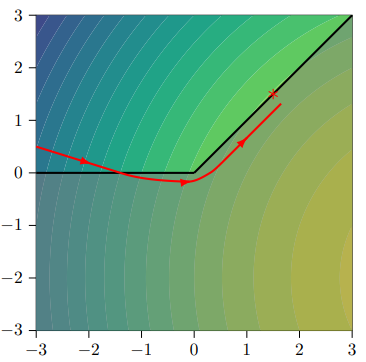
\includegraphics[width=.32\textwidth]{images/feedback_opt_08.png}
    \hfill
    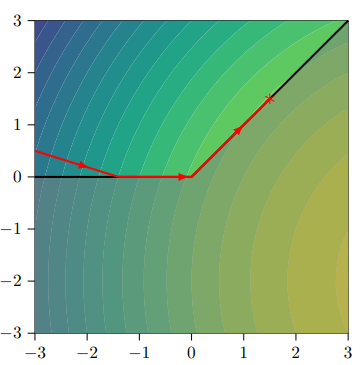
\includegraphics[width=.32\textwidth]{images/feedback_opt_09.png}
    \hfill
    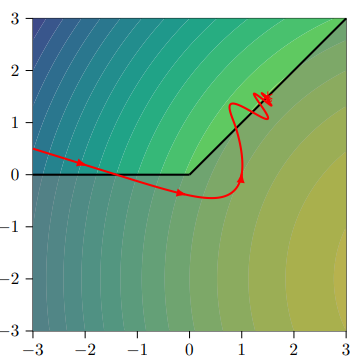
\includegraphics[width=.32\textwidth]{images/feedback_opt_10.png}
    \caption{Qualitative comparison of the trajectories produced by penalty, projected-gradient, and saddle-flow methods. Penalty methods may tolerate small constraint violations, projected-gradient methods maintain feasibility through projection, and saddle-flow methods approach feasibility asymptotically but may exhibit oscillatory behavior.}
    \label{fig:feedback-optimization-tradeoffs}
\end{figure}

In all cases, the same general message remains valid: feedback optimization does not require a full dynamical model of the plant, but it does require the right steady-state information. The central ingredients are the output measurements and the steady-state sensitivity matrix
\[
\nabla_u h(u;w),
\]
which together make it possible to embed optimization algorithms directly into the feedback loop.

\subsection{Extremum seeking}
\subsubsection{Extremum seeking}
So far, all feedback-optimization schemes relied on at least some approximate knowledge of the steady-state sensitivities
\[
\nabla_u h(u;w),
\]
or, equivalently, of the gradient of the performance map with respect to the input. In many applications, however, this information may be unavailable or too unreliable to be useful. This happens, for instance, when the plant is poorly modeled, when the operating conditions vary significantly over time, or when the steady-state map is known only through empirical performance charts.

This raises a natural question: can we optimize a steady-state performance index without any explicit knowledge of the gradient? Extremum-seeking control answers this question positively. It is a class of \emph{zeroth-order} optimization methods, meaning that it seeks the optimizer by using only measurements of the cost or performance, without requiring an analytical model of its gradient.

The general setting is the following. We consider again a fast stable plant, and we associate to each constant input $u$ a scalar performance metric
\[
J(u),
\]
which we want to minimize or maximize. The key difficulty is that the gradient
\[
\nabla_u J(u)
\]
is unknown. Extremum seeking overcomes this difficulty by injecting a small oscillatory perturbation into the input, observing the corresponding oscillatory component in the measured performance, and extracting from it an estimate of the local gradient.

This is why extremum seeking is often regarded as a learning-based feedback optimizer: it does not need a model of the steady-state sensitivities, because it estimates the necessary descent information online from measured data. In this sense, it complements the methods studied earlier in the chapter. When sensitivities are available, gradient, projected-gradient, or primal--dual methods are natural. When sensitivities are unknown, one may either estimate them or switch to a purely zeroth-order approach such as extremum seeking.

It is worth stressing one important robustness point. Even when the available sensitivity model is very inaccurate, the feedback-optimization schemes discussed previously may still work reasonably well. However, if one wants to avoid relying on such information altogether, extremum seeking is a natural alternative. This is one of the main motivations for introducing it at the end of the chapter.

\paragraph{Exercise.}
A useful fact to check is the following: both projected gradient descent and saddle-flow methods cannot have an equilibrium corresponding to an infeasible steady state
\[
y\notin\mathcal Y.
\]
This reinforces the idea that feedback optimization is structurally tied to feasibility. Extremum seeking, on the other hand, addresses a different issue: not the lack of feasibility mechanisms, but the lack of gradient information.

\subsubsection{Extremum-seeking architecture}

The simplest extremum-seeking idea can be explained for a scalar input. Suppose that the plant is fast and stable, and that the measured steady-state performance is $J(u)$. We want to optimize $J(u)$ without knowing its gradient.

The controller is built around four basic ingredients:
\begin{itemize}
    \item an \emph{exploration signal}, which perturbs the input with a small sinusoid;
    \item a \emph{high-pass filter}, which removes the slowly varying offset in the measured performance;
    \item a \emph{demodulation step}, which multiplies the filtered performance by a sinusoidal signal at the same frequency;
    \item a \emph{low-pass filter} followed by an integrator, which extracts an average descent direction and updates the nominal input.
\end{itemize}

Denoting by $\hat u_k$ the slowly varying nominal input and by $\rho \sin(\omega k)$ the injected perturbation, the actual plant input is
\[
u_k=\hat u_k+\rho \sin(\omega k).
\]
So the plant is continuously excited around the nominal operating point. The purpose of this small oscillation is to probe the local slope of the performance function.

The measured performance $J(u_k)$ is then passed through a high-pass filter, which removes the average component and keeps the oscillatory part induced by the perturbation. This signal is subsequently multiplied by a sinusoid of the same frequency. This multiplication step is often called \emph{demodulation}, because it extracts the component of the output that is correlated with the injected exploration signal. Finally, a low-pass filter removes the high-frequency terms, leaving only a slowly varying approximation of the gradient. The resulting signal is then integrated to update the nominal input $\hat u_k$ in the direction of improvement.

\begin{figure}[!h]
    \centering
    \begin{tikzpicture}[
    >=Latex,
    line width=1pt,
    font=\sffamily
]

%======================
% Top plant block
%======================
\draw (4.3,3.0) rectangle (8.2,5.0);
\node[align=center, font=\fontsize{11}{13}\selectfont] at (6.25,4.0) {(FAST) STABLE\\PLANT};

% Input to plant
\draw[->] (0.5,4.0) -- (4.3,4.0);
\node[above, font=\fontsize{9}{11}\selectfont] at (2.0,4.3) {input $u$};

% Output from plant
\draw[-] (8.2,4.0) -- (14.6,4.0);
\node[above, font=\fontsize{9}{11}\selectfont] at (10.4,4.3) {performance $J(u)$};

% Right vertical return
\draw[-] (14.6,4.0) -- (14.6,1.0);

%======================
% Bottom row blocks
%======================

% Summing node
\draw (1.2,1.05) circle (0.28);
\node at (1.2,1.05) {$+$};

% Integrator
\draw (2.4,0.2) rectangle (4.8,1.9);
\node[align=center, font=\fontsize{9}{11}\selectfont] at (3.6,1.32) {INTEGRATOR};
\node[align=center, font=\fontsize{8}{10}\selectfont] at (3.6,0.73)
{$\hat{u}_{k+1}=\hat{u}_{k}-\delta u_k$};

% Gain triangle (left-pointing)
\node[
    draw,
    isosceles triangle,
    isosceles triangle apex angle=60,
    shape border rotate=180,
    minimum height=1.2cm,
    minimum width=1.0cm,
    inner sep=0pt
] (gain) at (6.2,1.05) {};
\node[font=\fontsize{9}{11}\selectfont] at (5.98,1.05) {$\alpha$};

% Low-pass filter
\draw (6.9,0.2) rectangle (9.1,1.9);
\node[align=center, font=\fontsize{9}{11}\selectfont] at (8.0,1.32) {LOW-PASS};
\node[align=center, font=\fontsize{9}{11}\selectfont] at (8.0,0.78) {FILTER};

% Multiplier
\draw (10.1,1.05) circle (0.28);
\node at (10.1,1.05) {$\times$};

% High-pass filter
\draw (11.1,0.2) rectangle (13.7,1.9);
\node[align=center, font=\fontsize{9}{11}\selectfont] at (12.4,1.32) {HIGH-PASS};
\node[align=center, font=\fontsize{9}{11}\selectfont] at (12.4,0.78) {FILTER};

%======================
% Connections
%======================

% Right return into high-pass
\draw[->] (14.6,1.0) -- (13.7,1.0);

% High-pass to multiplier
\draw[->] (11.1,1.05) -- (10.38,1.05);

% Sine input to multiplier
\draw[->] (10.1,-0.75) -- (10.1,0.77);
\node[below, align=center, font=\fontsize{8}{10}\selectfont] at (9.45,-0.05)
{$\dfrac{2}{\rho}\,\sin(\omega k)$};

% Multiplier to low-pass
\draw[->] (9.82,1.05) -- (9.1,1.05);

% Low-pass to gain
\draw[->] (6.9,1.05) -- (6.5,1.05);
\node[above, font=\fontsize{9}{11}\selectfont] at (5.2,1.2) {$\delta u$};

% Gain to integrator
\draw[->] (5.38,1.05) -- (4.8,1.05);

% Integrator to summing node
\draw[->] (2.4,1.05) -- (1.48,1.05);
\node[above, font=\fontsize{9}{11}\selectfont] at (2.0,1.38) {$\hat{u}$};

% Sine input to summing node
\draw[->] (1.2,-0.75) -- (1.2,0.77);
\node[left, font=\fontsize{8}{10}\selectfont] at (0.95,-0.05) {$\rho\,\sin(\omega k)$};

% Summing node to plant input path
\draw[-] (0.45,1.05) -- (0.45,4.0);
\draw[->] (0.45,1.05) -- (0.92,1.05);

\end{tikzpicture}
    \caption{Basic extremum-seeking architecture. A small sinusoidal perturbation is added to the nominal input $\hat u_k$ in order to explore the local slope of the steady-state performance $J(u)$. The measured performance is high-pass filtered, demodulated, low-pass filtered, and finally integrated so as to generate an update of the nominal input.}
    \label{fig:extremum-seeking-architecture}
\end{figure}

The exploration signal
\[
\rho \sin(\omega k)
\]
should be thought of as a deliberate excitation used to reveal local gradient information. The demodulation signal, typically proportional to
\[
\frac{2}{\rho}\sin(\omega k),
\]
is chosen so that, after averaging, the product isolates the first-order term of the Taylor expansion of the performance function.

So the overall architecture can be interpreted as a feedback mechanism that reconstructs a gradient estimate from input--output oscillations, without ever requiring an explicit model of the plant or of the performance map.

\subsubsection{Why extremum seeking behaves like gradient descent}

The basic mechanism can be understood with a first-order Taylor expansion. Starting from
\[
u_k=\hat u_k+\rho \sin(\omega k),
\]
assume that $\rho$ is small, so that the performance function can be expanded around the nominal input:
\[
J(u_k)\approx J(\hat u_k)+\nabla_u J(\hat u_k)\,\rho \sin(\omega k).
\]
The first term is a slowly varying offset, while the second is an oscillatory term whose amplitude is proportional to the unknown gradient.

After the high-pass filter, the offset is removed, and we are left approximately with
\[
\nabla_u J(\hat u_k)\,\rho \sin(\omega k).
\]
The next step is demodulation. Multiplying by
\[
\frac{2}{\rho}\sin(\omega k)
\]
gives
\[
\nabla_u J(\hat u_k)\, 2\sin^2(\omega k).
\]
Using the identity
\[
2\sin^2(\omega k)=1-\cos(2\omega k),
\]
we see that this signal consists of a constant part,
\[
\nabla_u J(\hat u_k),
\]
plus a fast oscillation at frequency $2\omega$. The low-pass filter removes the oscillatory component and keeps only the average value. Therefore, after the low-pass filter, the signal is approximately
\[
\nabla_u J(\hat u_k).
\]

If this signal is then multiplied by a gain $\alpha$, we obtain the update direction
\[
\delta u_k=\alpha \nabla_u J(\hat u_k).
\]
Finally, the integrator implements
\[
\hat u_{k+1}=\hat u_k-\delta u_k,
\]
hence
\[
\hat u_{k+1}=\hat u_k-\alpha \nabla_u J(\hat u_k).
\]
But this is exactly the gradient-descent iteration.

So, at an intuitive level, extremum seeking is nothing but gradient descent in disguise:
\begin{itemize}
    \item the exploration signal reveals the local slope of the performance map;
    \item the filtering and demodulation reconstruct the gradient;
    \item the integrator performs the actual descent step.
\end{itemize}

Of course, this derivation is only a sketch. A rigorous analysis requires averaging arguments, time-scale separation, and assumptions on the filters and on the plant dynamics. But the basic idea is exactly the one above: extremum seeking creates its own gradient information through oscillatory probing.

\subsubsection{Applications of extremum seeking}

Extremum seeking is especially attractive in applications with the following features:
\begin{itemize}
    \item the plant is fast and stable at the time scale of the optimizer;
    \item the steady-state performance map is poorly known or strongly parameter dependent;
    \item the optimization problem is low dimensional;
    \item small oscillatory perturbations of the input are acceptable.
\end{itemize}

A classical example is photovoltaic maximum-power-point tracking. In a photovoltaic system, the active power generated by the panel depends on the operating voltage, and the power--voltage curve changes significantly with solar irradiance and temperature. Therefore, the location of the optimal voltage is not fixed and may vary continuously during operation. Moreover, an accurate model of the full dependence on the environmental variables may be difficult to maintain online.

In this situation, extremum seeking is very natural. By slightly perturbing the voltage and measuring the resulting power, the controller can estimate whether the current operating point is to the left or to the right of the maximum, and then move the nominal voltage in the correct direction. In this way, the controller tracks the operating voltage that maximizes active power generation without requiring an explicit gradient model.

This is a particularly good use case because:
\begin{itemize}
    \item the optimum varies with exogenous conditions;
    \item the model is poor or uncertain;
    \item the control input is low dimensional;
    \item the actuator cost of a small oscillatory probing signal is acceptable.
\end{itemize}

Other relevant applications include internal combustion engines, chemical processes, compressor systems, and meta-optimization problems such as tuning controller parameters. In all these cases, extremum seeking is valuable when the optimizer can rely on measured performance only, while the gradient or the steady-state sensitivity is unavailable.

\paragraph{Final perspective.}
This closes the chapter with an important conceptual message. Feedback optimization can be organized along a spectrum:
\begin{itemize}
    \item if reliable steady-state sensitivities are available, one can use gradient, projected-gradient, or primal--dual schemes;
    \item if sensitivities are inaccurate, one may still rely on robust feedback optimization based on approximate models;
    \item if sensitivities are completely unknown, one can move to learning or zeroth-order methods such as extremum seeking.
\end{itemize}

So extremum seeking is not a separate topic disconnected from the rest. It is the natural endpoint of the feedback-optimization viewpoint: when model-based gradient information disappears, the controller can still recover optimization directions directly from feedback measurements.